\documentclass{article}
\usepackage[utf8]{inputenc}
\usepackage{algorithm}
\usepackage{algpseudocode}
\usepackage{amssymb}
\usepackage{amsmath}
\usepackage{graphicx}

\title{Componenti Connesse e MST}
\author{Luca Maltempo}
\date{October 2021}

\begin{document}

\maketitle

\section{Introduzione}
Un grafo è caratterizzato da un insieme di vertici e di archi che li uniscono. Sul grafo sono possibili diverse operazioni, in questo caso ci occuperemo della ricerca delle componenti connesse di un grafo e della ricerca dell'albero di connessione minimo (MST). Esistono diverse applicazioni reali che richiedono il calcolo di queste due operazioni su grafi molto grandi, quindi, è necessario che gli algoritmi implementati siano veloci anche all'aumentare della grandezza del grafo.
\section{Cenni Teorici}
\subsection{Grafo}
Per memorizzare un grafo è necessario mantenere in memoria l'insieme di nodi e i diversi archi che collegano i nodi del grafo, per fare questo è stata utlizzata la matrice di adiacenza. In particolare, i grafi creati sono non orientati e pesati, ovvero ogni arco che collega due nodi è caratterizzato da un peso scelto casualmente.
\subsection{Union Find}
Le Union Find sono delle strutture dati per insiemi disgiunti. Ogni insieme è identificato da un unico rappresentante, Si possono eseguire tre diverse operazioni:
\begin{itemize}
    \item Make-Set(x): Crea un insieme contente un unico elemento x.
    \item Find-set(x): Restituisce il rappresentante dell'insieme contenente x.
    \item Union(x,y):  Unisce i due insiemi, modifica il rappresentante in modo che questo sia lo stesso tra tutti gli elementi dell'insieme.
\end{itemize}
Per implementare le Union-Find è sono state usate delle liste doppiamente concatenate. Ogni lista rappresenta un insieme disgiunto, ogni nodo della lista contiene l'elemento dell'insieme, un riferimento al prossimo elemento e infine un riferimento al rappresentante dell'insieme. Le prime due operazioni della Union-Find sono banali e hanno costo costante, Union(x,y) invece è una operazione costosa poichè richiede la modifica del rappresentante di tutti gli elementi del secondo insieme che viene unito al primo. Un'euristica utile a velocizzare questo processo prevede semplicemente la concatenazione della lista con meno elementi alla lista con più elementi in modo tale che sia necessario modificare il minor numero di riferimenti al rappresentante possibile.  Attraverso un'analisi aggregata per una sequenza di m operazioni su n elementi si ottiene un tempo per Union di $O(m+n log{} n)$ .
\subsection{Componenti Connesse}
Dato un grafo G=(V,E) le sue componenti connesse sono i sottoinsiemi disgiunti di V tali che ogni sottoinsieme contenga i vertici che possono essere raggiunti l'uno dall'altro. Quindi due nodi appartengono alla stessa componente connessa se e solo se esiste un cammino che li unisce. Per trovare le componenti connesse di un grafo si usa un algoritmo basato sulle Union-Find: 
\begin{algorithm}
\caption{ComponentiConnesse(G)}\label{alg:cap}
\begin{algorithmic}
\For{\texttt{ogni vertice $v$ $\in$ $G.V$}}
    \State \texttt{Make-Set($v$)}
\EndFor
\For{\texttt{ogni arco $(u,v)$ $\in$ $G.E$}}
    \If{Find-Set($u$) $\neq$ Find-Set($v$)}
        \State Union($u,v$)
    \EndIf
\EndFor
\end{algorithmic}
\end{algorithm}
\\
Il costo temporale di ComponentiConnesse(G) dipende dall'implementazione di Union-Find, come illustrato nella sezione risultati sperimentali l'algoritmo ha un costo lineare con l'aumentare dei nodi e archi del grafo.

\pagebreak[4]

\subsection{MST}
Dato un grafo G=(V,E) non orientato e pesato è possibile trovare un albero di connessione minimo, ovvero un cammino formato da V-1 archi che unisca tutti i nodi del grafo, abbia costo minimo e non presenti cicli. Per fare questo è stato implementato l'algoritmo MST-Kruskal :
\begin{algorithm}
\caption{MST-Krukal(G,w)}\label{alg:cap2}
\begin{algorithmic}
\State \texttt{A $\xleftarrow[]{}$ $\emptyset$}
\For{\texttt{ogni vertice $v$ $\in$ $G.V$}}
    \State \texttt{Make-Set($v$)}
\EndFor
\State \texttt{ordina gli archi di $G.E$ in senso non decrescente rispetto al peso w}
\For{\texttt{ogni arco $(u,v)$ $\in$ $G.E$}}
    \If{Find-Set($u$) $\neq$ Find-Set($v$)}
        \State \texttt{A $\xleftarrow[]{}$ A $\cup$ \{(u,v)\}}
        \State \texttt{Union($u,v$)}
    \EndIf
\EndFor
\end{algorithmic}
\end{algorithm}
\\
Come per ComponentiConnesse(G) anche l'algoritmo di Kruskal per la ricerca dell'albero di connessione minimo ha un tempo di esecuzione lineare al crescere dei nodi e archi del grafo.

\section{Esperimenti svolti}
Per testare gli algoritmi delle componenti connesse e del MST sono stati generati casualmente grafi di diverse dimensioni, il più piccolo presenta solo 2 nodi e il più grande 4096, i grafi aumentano di dimensione seguendo la potenza del 2. Ogni grafo, fissata la dimensione, presenta 5 versioni, ognuna con una probabilità di arco tra due nodi differente. Per ogni grafo generato verranno ricercate le componenti connesse e si misurerà il tempo necessario per completare l'operazione, infine, per i grafi che presentano una sola componente connessa sarà possibile applicare l'algoritmo di Kruskal, anche in questo caso si raccoglieranno i diversi tempi di esecuzione al variare della dimensione del grafo e della probabilità di arco. 

\section{Risultati sperimentali}

A seguire si possono vedere le tabelle che riportano i risultati dell'algoritmo per la ricerca delle componenti connesse al variare del numero di nodi nel grafo e della probabilità  p di arco tra due nodi. Viene riportato anche il grafico che mostra il tempo di esecuzione di ComponentiConnesse(G) con probabilità di arco $p = 0.8$. 

\begin{tabular}{ |p{1.5cm}|p{1.5cm}|p{1.5cm}|p{1.5cm}|p{1.5cm}|p{1.5cm}| }
 \hline
 \multicolumn{6}{|c|}{Numero di Componenti Connesse} \\
 \hline
    Nodi & p = 0.2 & p = 0.4 & p = 0.6 & p = 0.8 & p = 1 \\
 \hline
    2 & 2 & 1 & 2 & 1 & 1 \\
    4 & 4 & 2 & 1 & 1 & 1 \\
    8 & 3 & 1 & 1 & 1 & 1 \\
    16 & 2 & 1 & 1 & 1 & 1\\
    32 & 1 & 1 & 1 & 1 & 1\\ 
    ... & ... & ... & ... & ... & ...\\
    4096 & 1 & 1 & 1 & 1 & 1\\
 \hline
\end{tabular}

\medskip

\begin{tabular}{ |p{1.5cm}|p{1.5cm}|p{1.5cm}|p{1.5cm}|p{1.5cm}|p{1.5cm}| }
 \hline
 \multicolumn{6}{|c|}{Tempo ComponentiConnesse(G) in secondi} \\
 \hline
    Nodi & p = 0.2 & p = 0.4 & p = 0.6 & p = 0.8 & p = 1 \\
 \hline
    16 & 0.00000 & 0.00000 & 0.00000 & 0.00000 & 0.00100 \\
    32 & 0.00000 & 0.00000 & 0.00000  & 0.00000 & 0.00000 \\
    64 & 0.00100 & 0.00100 & 0.00100 & 0.00100 & 0.00199 \\
    128 & 0.00199 & 0.00200 & 0.00399 & 0.00499 & 0.00598 \\
    256 & 0.015 & 0.010 & 0.014 & 0.019 & 0.020 \\
    512 & 0.024 & 0.052 & 0.055 & 0.073 & 0.088 \\
    1024 & 0.13 & 0.21 & 0.24 & 0.28 & 0.34\\ 
    2048 & 0.52 & 0.90 & 1.01 & 1.11 & 1.48\\
    4096 & 1.80 & 2.85 & 4.30 & 4.54 & 5.75\\
 \hline
\end{tabular}

 \begin{figure}[h]
     \centering
     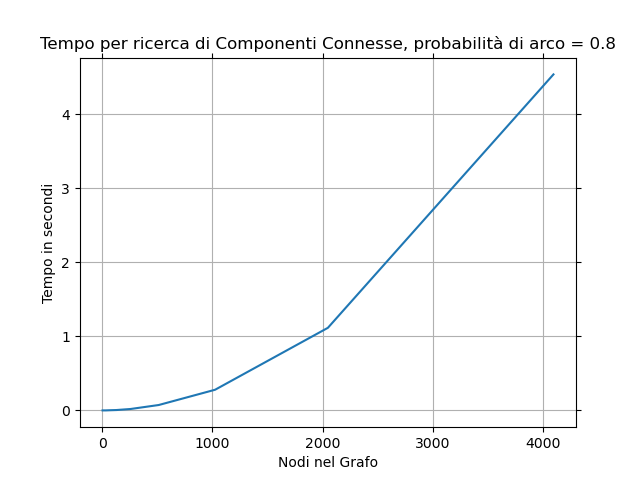
\includegraphics[scale=0.75]{tempiCCProb0.8.png}
     \label{fig:tempiCC08}
 \end{figure}
\pagebreak[4]
A seguire è riportata la tabella che mostra il tempo di esecuzione di MST-Kruskal al variare del numero dei nodi e della probabilità p di arco tra nodi. Inoltre si riporta sotto forma di grafico il legame tra tempo di esecuzione di MST-Kruskal e aumento del numero dei nodi del grafo con $p = 0.8$.

\medskip
\medskip

\begin{tabular}{ |p{1.5cm}|p{1.5cm}|p{1.5cm}|p{1.5cm}|p{1.5cm}|p{1.5cm}| }
 \hline
 \multicolumn{6}{|c|}{Tempo MST-Kruskal(G,w) in secondi} \\
 \hline
    Nodi & p = 0.2 & p = 0.4 & p = 0.6 & p = 0.8 & p = 1 \\
 \hline
    16 & - & 0.00000 & 0.00000 & 0.00000 & 0.00000 \\
    32 & 0.04289 & 0.00100 & 0.00000  & 0.00000 & 0.00000 \\
    64 & 0.00100 & 0.00100 & 0.00200 & 0.00299 & 0.00299 \\
    128 & 0.00299 & 0.00499 & 0.00598 & 0.00698 & 0.00798 \\
    256 & 0.011 & 0.017 & 0.019 & 0.034 & 0.034 \\
    512 & 0.049 & 0.071 & 0.090 & 0.128 & 0.144 \\
    1024 & 0.17 & 0.28 & 0.43 & 0.49 & 0.57\\ 
    2048 & 0.68 & 1.18 & 1.40 & 2.25 & 2.47\\
    4096 & 2.37 & 4.50 & 6.42 & 8.51 & 9.65\\
 \hline
\end{tabular}

 \begin{figure}[h]
     \centering
     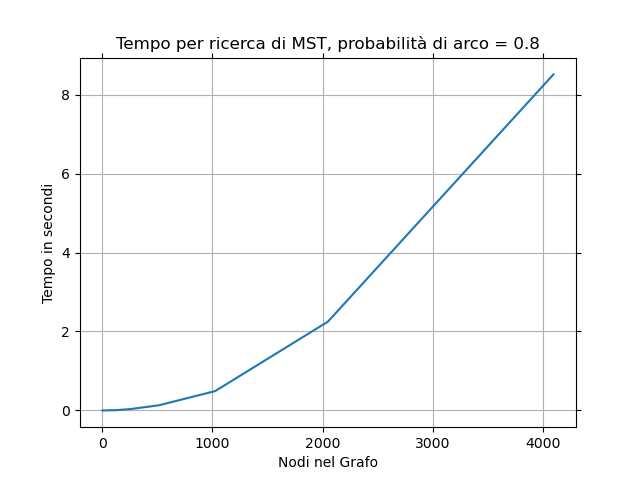
\includegraphics[scale=0.75]{tempiMSTProb0.8.png}
     \label{fig:tempiMST08}
 \end{figure}
 
 Come si vede dalle tabelle e dai due grafici entrambi gli algoritmi implementati attraverso la struttura dati Union-Find con lista concatenata hanno un tempo di esecuzione lineare al crescere dei nodi del grafo.
 
\end{document}
